\chapter{考察}
%研究全体の考察
\begin{comment}
  \section{バッファのとりこぼしについて}

  既知の問題としては,Nexus7が録音中に頻繁にバッファを取りこぼすことが挙げられる.

  %![](img/nexus7_is_bad.png)

  この現象によりパルスが到来した時刻が分からないので,上記手法が使えなかった.
  原因はハードウェアにあるのかOSにあるのかブラウザの実装にあるのか不明であり,現在調査中である.
  MacBookAirとMacBookPro間では同期に成功している.



  他には,TDMAのみではN回の排他的パルス送信が必要で同期に時間がかかるという問題がある.
  これにはスペクトル拡散を使っているのでCDMA(Code Division Multiple Access)化できる余地があるが,
  今までの実験で,Nexus7ではGold符号でBPSKした信号が重なったときに,
  分離検出できないという問題があったため,開発は滞っている.

\end{comment}



本研究で狙いとするスマートデバイスを用いた音像定位手法に必要な,高精度な同期・測距を提案手法によって実現できた.
また,同期した複数端末による音像定位は,同一の音源として聞かせることができた.

受聴者からみた三角形のみかけの幅が大きい場合にASWが増加したのは,
ASWの要因である二つのノード間で両耳間相関度(ICC: interaural cross-correlation)が
%不可干渉
%インコヒーレントだからだと考えられる<<要出典>>.
小さかった\cite{morimoto95},もしくは,初期側方エネルギー率が大きい,
つまり直接音の入射角度に対して垂直な成分の音圧レベルと直接音の音圧レベルの比が大きかった\cite{barron81}
と考えられる.
%という要因<<要出典>>も考えられる.
また,
三角形の内側の受聴者がLEVを体験したのは,
LEVの要因である前後エネルギー比\cite{suehiro06}
が小さくなったからと考えられる.




\section{同期制御のネットワーク構成について}

以前はP2PリングネットワークChordアルゴリズム\cite{chordalg, SHAKER}を用いて,相関演算を各端末に任せることで,並列計算を行い,計算量の削減を狙っていた(図\ref{fig:scheduling}).
また,このリングをトークンリングとして用いることで,パルスの排他制御を行っていた.
しかし,少数端末での実験状況下において,パルス同定アルゴリズムのデバッグのしやすさの観点から、各端末に計算を分散して並列化による計算時間を削減するよりも、
一台のパソコンで処理したほうが結果が比べやすいという開発上の観点から,現在は計算サーバーを導入している.
%また、以前計算が停止した原因は私の書いたプログラムにゼロ除算を含む計算が生じる可能性があたったためで、nexus7でも計算自体は可能です。


\begin{figure}[p]\centering
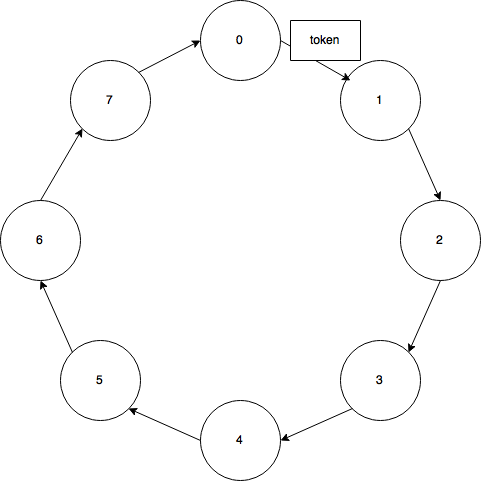
\includegraphics[clip,width=0.85\hsize]{img/chord_ring_network.png}
\caption{ネットワーク上でのトークンパッシング}\label{fig:scheduling}
\end{figure}




\section{ダイレクトパスが存在しない時の回折パルス検出の問題}

端末間に障害物があると音波が回折して伝搬する.また,コンクリート壁などの反射波の方がエネルギー大きくなる,非線形歪みの影響\cite{nonlinear}など,ダイレクトパスがない時には同期性能が落ちる問題がある.
微弱な先行波を捉える必要があるが,非線形歪みと反射音,回折音をどう区別するかの問題が残っている.
ハードウェアや環境に応じて2端末間のインパルス応答は毎回異なるため識別は困難である.

この問題に対しては,同期回数を増やして統計的な処理を行えば,この問題に対して解決作を見出せる可能性がある.
パルス交換の試行回数を増やし,一回の計測に必要な時間を減らすことができれば,実用に耐えるものになるだろう.




\section{相対位置推定結果が回転・反転する問題}

問題設定上,回転や鏡面反転した解が出てきてしまう.
これは,相対位置を推定している以上防ぐことができない.
そのため,ユーザが手動で修正するためのUIを実装する必要がある.
他にも,3台の端末の位置を固定し,推定から外すことで,回転・反転を防ぐことができる.



\section{相対位置推定アルゴリズムの解が収束しない問題}

相対位置推定の結果が現実の位置を反映できていない問題がある.
これは,最急降下法の解が収束していないのが原因である.
使用する反復解法に最急降下法よりも解の探索範囲が広いガウス・ニュートン法や共役勾配法などを導入する,
あるいは多次元尺度構成法を導入する,などの解決策が考えられる.






\section{システムクロック校正}
システムクロックの差に依存して同期が次第にずれていく問題がある.
端末のシステムクロックの進みかたはハードウェアごとにわずかに異なる.
そのため,同期してから長時間経つと,次第に端末間で遅延が生じる.
これは,同一音源を同期的に再生し続けることで,次第にずれが聞き取れるようになることを意味する.
この遅延を検出する手法について述べる.
解決手法として,2端末間でパルスをやりとりしてサンプリング数の差を計測する手法が提案されている\cite{tpsn}.

端末 A のクロックを $S_A$,
端末 B のクロックを $S_B$ して,
時刻 $t$ 後に
A のサンプル数が $i$ ,
B のサンプル数が $i+d$ だけ異なっているとする.
このとき,Aを基準とした遅延比率 $S_B/S_A$ を求める.

\begin{figure}[p]\centering
  \hspace{-2mm}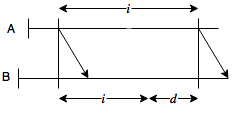
\includegraphics[clip,width=1.1\hsize]{img/phase_shift2.png}
  \caption{再同期}\label{fig:phaseshift2}
\end{figure}

図\ref{fig:phaseshift2}より
$$\begin{aligned}
\frac{i}{S_A} &= \frac{i+d}{S_B} = t \\
\frac{S_B}{S_A} &= \frac{i+d}{i}
\end{aligned}$$
である.

遅延の検出は,端末間の相対距離に変化がない限り,
端末Aが端末Bへとパルスを発生するだけで良く,
端末BはAへと返答パルスを返す必要はない.
端末Aと端末Bは同期済みのため,伝搬時間は既知であるからである.









\section{音圧校正}
スマートデバイス毎にマイクロホンやスピーカのアンプ出力は異なるため,DBAP法は使えない.
機器間での音圧校正にはいくつかの手法が提案されている\cite{和泉洋一, 澤上佳希}.
ここでは,機器ごとの音圧を校正する手法を示す.

LTI(線形時不変)システムを仮定する.
$N$ 台の端末の番号を $i,j \in \{1\dots N\}$ とする.
端末 $i$ から端末 $j$ への信号伝達を考える.
$e$ を端末 $i$ で生成した単位振幅,
$v_i$ を端末 $i$ のスピーカアンプの増幅係数,
$m_j$ を端末 $j$ のマイクロホンアンプの増幅係数,
$d_{ij}=d_{ij}$ を $ij$ 間の測定距離,
$x_{ij}$ を $j$ が観測した $i$ からの信号の振幅とする.
音波の振幅は距離に反比例して減衰することが知られているので,
音声信号の伝達は

\begin{figure}[p]\centering
  \hspace{-2mm}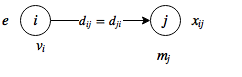
\includegraphics[clip,width=1.1\hsize]{img/sound_pressure_calibration.png}
  \caption{soundpressurecalibration}\label{fig:soundpressurecalibration}
\end{figure}

$$
e v_i \frac{1}{d_{ij}} m_j = x_{ij}
$$

とモデル化できる(図\ref{fig:soundpressurecalibration}).
このとき,ある端末 $k$ の出力係数 $v_k$ と他の端末 $i$ の出力係数 $v_i$ との比 $v_i/v_k$ を求める.

$$
e v_i m_j = x_{ij}d_{ij}
$$

なので

$$\begin{aligned}
\frac{e v_j m_j}{e v_k m_j} &= \frac{x_{ij} d_{ij}}{x_{kj} d_{kj}} \\
\frac{v_j}{v_k} &= \frac{x_{ij} d_{ij}}{x_{kj}d_{kj}} \\
\end{aligned}$$

である.
観測した振幅 $x_{ij}$ および測定距離 $d_{ij}$ は誤差を含むので,
それらを平均した $\hat{v_i}$ は

$$
\frac{\hat{v_i}}{v_k} = \frac{1}{N} \sum_{i\neq j \neq k} \frac{x_{ij} d_{kj}}{x_{kj}d_{ij}} \\
$$

と定義できる.$d_{ii}$ のときは距離が0となりゼロ除算が発生するので,
$i\neq j \neq k$ としている.

一番出力の低い端末 $k$ の出力係数 $v_k$ を基準とすることで,
すべての端末において定格出力を守ることができる.

スピーカの出力特性は周波数帯域によって異なるが,
チャープ信号などを利用して得られた信号に対してこのモデルを利用すれば,互いのマイクロホン係数とスピーカ係数が求められると考えられる.
このモデルが成り立つか実験が必要である.





\section{パルス検出できない端末間の問題}
端末間距離が遠いなどの理由で互いにパルスのやりとりができない問題がある.
互いの信号を検出できなかったノード間での校正を考える.
図\ref{fig:nt}に隣接ノードではない端末を含むネットワークを示す.


\begin{figure}[p]
  \centering
  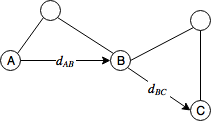
\includegraphics[clip,width=1.05\hsize]{img/network_topology.png}
  \caption{中継ノード}\label{fig:nt}
\end{figure}

このとき端末 A と端末 C 間では同期・測距ができていないが,
互いに端末 B とは同期・測距できているという状況である.



\section{パルス検出できない端末間での同期・クロック校正}

中継となる端末を設定し,多段同期すればよい.
時刻の基準となる
端末 $A$ がパルスを発した時間を $t_{AA}$ として
そのパルスが端末 $B$ に届いた時間は $t_{AB}$ とする.
また,
端末 $B$ がパルスを発した時間を $t_{AB}$ として
そのパルスが端末 $C$ に届いた時間は $t_{BC}$ とする.
そしてそれぞれの伝達時間を $d$ とすると図\ref{fig:rd}のようになる.


\begin{figure}[p]
  \centering
  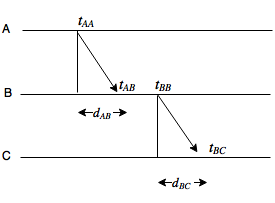
\includegraphics[clip,width=1.05\hsize]{img/rel_delay.png}
  \caption{パルス検出できない端末間での同期}\label{fig:rd}
\end{figure}

このとき,まず端末 $C$ は端末 $B$ と同期して,
その後端末 $B$ と端末 $A$ の時刻ずれ情報をもとにさらに端末 $A$ との同期ができる.

この手法を用いれば,クロック校正も多段校正できる.
多段的な同期・クロック校正が可能であるかについても,要実験である.

\section{パルス検出できない端末間での音圧校正}
音圧校正も多段校正できる.


端末 $A$ を基準に音圧校正を考えると

$$
\frac{v_B}{v_A} = \frac{x_{iB} d_{iB}}{x_{AB}d_{AB}} \\
\frac{v_C}{v_B} = \frac{x_{iC} d_{iC}}{x_{BC}d_{BC}} \\
$$

であるので

$$
\frac{v_C}{v_A} =
\frac{v_B v_C}{v_A v_B} =
\frac{x_{iB} x_{iC} d_{iB} d_{iC}}{x_{AB} x_{BC} d_{AB} d_{BC}}
$$

とすれば端末 A と端末 C の出力比率を求められる.







\section{パルス回数の問題}

現在の提案手法では同期に時間がかかるのでリアルタイム同期を目指す.
N台の同期にN回パルス必要という問題もある.
解決手法として,TDMAだけでなくGold符号を用いたCDMAも試みた.
シミュレーションでは2つの異なる信号が重なる状況下においても機能したが,
現実空間で試すとパルスが重なったときに信号をうまく分離できない問題があった.
これも拡散符号の非線形歪みの影響と考えられる.

ところで,測距のみを行い,音圧校正と同期を考えなければ,パルスは3台が1回ずつ放つだけで十分である.
これはGPSと同じ仕組みであり,3台の端末の相対位置が取得できれば,
他の端末はその3台からの相対距離に応じて三角測量の要領で相対位置が算出できるからである.
この手法に合わせて同期手法を提案手法とは異なる結合振動子系\cite{合原一究, 谷口義明, 木村宏人}のような適応的アルゴリズムにすることで,システムクロックのずれにも対応できるようになる.
しかし音圧校正のためには,現在の手法では全ての端末が音を出す必要がある問題が残されている.



\section{位置変更による再同期の必要性}

端末が動くと再同期が必要という問題もある.
この原因は同期と測距を同時にしているからである.
逆に言えば,測距と同期とは別の手法を用いればよい.
例えば,GPSと同じように,位置固定した連続パルス発信端末を導入すればよい.
これにより,リアルタイム測距は可能になる.
同期に関してはも結合振動子系のような適応的なアルゴリズムを採用すれば,システムクロックのずれにも対応できる.
しかし,音圧校正のためには現在の手法では全ての端末が音を出す必要がある問題が残されている.



\section{計算量・計算時間削減のための最適化}
相互相関の計算に離散フーリエ変換ではなく離散コサイン変換を使うことで計算量を削減できる可能性がある.
しかし,高速離散フーリエ変換を高速離散コサイン変換に置き換えたことによる計算量の削減は高々O(n)であり,負荷改善のために導入する段階ではないと考える.


\section{システムの応用}
このシステムの応用例はいくつか考えられる.

例えば,仮想的な音像を動的に移動させられるという機能は,
音のみによる幽霊のような存在感を提示する効果を実現できる.
この効果を用いることで,リアルタイムで話す話者の発話の位置を,
群衆の特定の場所に配置するようなこともできると考えられる.
リアルタイム音声配信を提案システムに実装する場合,
発話者がマイクに話した音と実際にスピーカアレイから音がでるまでに時間差が生じるので,
発話者がスピーカアレイの中にいる場合は,少々話しづらいかもしれない.

また,同期的に端末が制御できるという機能を用いれば,
ライブ会場においてスマートデバイスをスマートサイリウムとして使うこともできる.
これは,スマートデバイスのディスプレイに色を発光させることでサイリウムの代理とし,
さらにその色を位置に応じて動的に変化させることで,甲子園高校野球で某学園が行っている色付きパネルを用いた人文字のような効果を演出できる.

他にも,同期的に音を鳴らせるという機能を利用すれば,
複数のスマートデバイスの音圧を合成してひとつの大きなアンプ出力のスピーカとして使うこともできる.
この利用例として,ストリートダンスの練習者がその場に集まった人々のスマートデバイスを用いることで,
専用の携帯式アンプ機器を持ち歩く必要なく大出力の音源を得ることができる.
こ場合,スピーカアレイのASWやLEVが大きくなる現象は,むしろライブ会場の臨場感を得ることができるため利点と言えるようになる.



\section{まとめ}
本章では実装したシステムの問題点とその解決策について触れた.
さらに,システムの実世界での応用例も述べた.
上記の解決策をひとつひとつ検証し実装していくことで,提案システムはより実用に耐えうるものになると言える.
